\documentclass{imc-inf}

\title{Data Mining in Sports}
\subtitle{Implementation and analysis of machine learning prediction models to find potential influential factors in results of matches in the Australian Football League}
\thesistype{Bachelor Thesis} % or Bachelor Expos\'e
\author{Thomas Gallagher}
\supervisor{Dr. Deepak Dhungana }
\copyrightyear{2023}
\submissiondate{02.04.2023}
\keywords {Data Analytics, Machine Learning, Sports Prediction, Neural Network}


\usepackage{listings}
\usepackage{subcaption}


\begin{document}
	\frontmatter\maketitle{}
	
	
	\begin{declarations}\end{declarations}
	
	
	
	\begin{abstract}
		Despite the large amounts of data produced by the sporting industry every year, there has been relatively little crossover between academic data science and professional sports. On the other hand, Data Mining techniques such as Machine Learning, Neural Networks and Association Methods, have seen rapid increases in their complexity and use over a wide variety of fields and disciplines. 
		This paper aims to address this issue of a lack of data science applications in sports, with regards to the Australian Football League (AFL), by applying Data Mining techniques to improve upon already utilised data analysis techniques present in modern professional sports. In this paper statistics and results from the previous 10 AFL seasons will be assessed to identify key features and possible trends and use them to create more explainable white box prediction models. This will help not only sports professionals and data scientists but also casual viewers to understand the finer statistical details behind sports.
		
	\end{abstract}
	
	
	
	\addtoToC{Table of Contents}%
	\tableofcontents%
	\clearpage
	
	
	\addtoToC{List of Tables}%
	\listoftables
	
	
	%   MAIN MATTER  %%%%%%%%%%%%%%%%%%%%%%%%%%%%%%%%%%%%%%%%%%%%%%%%%%%%%%%%%%%%%%
	\mainmatter%
	
	\chapter{Introduction}\label{chap:introduction}
	
	This paper will apply Data Mining techniques on Australian Rules Football data in an attempt to identify any trends that may occur in individual seasons and then further apply this information into a Neural Network to create a prediction model for subsequent games.
	
	The field of Data Mining has seen a rapid increase as we enter the digital age dominated digital information also commonly known as data. While many believe data mining to simply be the extraction of data it is actually a much broader topic. Data extraction is only the first step in data mining, the goal of data mining is to extract ‘previously unknown’ and unseen patterns from this data \cite{website:TechGuy}, much of which would be impossible to uncover without the help of computer systems. Data Mining is most commonly applied in commercial business. There it can be used to ‘help identify and predict individual and aggregate behaviour’ \cite{ACM}, or more commonly to predict how customers will consume/buy products and their buying habits so that they can more efficiently market their products in specific situations. Data Mining in sports however is much less advanced, despite massive amounts of data being produced by the sporting industry, it is mainly kept behind closed doors, with much of it focusing on player and team performance.
	\newline
		
	Although it is a quite unrepresented research area, there have been some recent attempts at data mining in sports, which have been used in a variety of areas including, classification \cite{Displays}, action recognition \cite{AEJ} and image recognition \cite{Heliyon}. While data mining has also been used to aid in the creation of sports prediction models \cite{CollegeFootball}\cite{Basketball}\cite{LSTMPrediction}, none of these models aim to identify trends within the sports apply these as part of their prediction model. 
	
	An issue with many prediction models is the lack of transparency in their decision making, a key concept of this is issue is the idea of black box and white box models. Black Box models are in most cases more accurate than white box model but much more difficult to interpret, the internal decisions and processes of the algorithms are much more difficult to extract, resulting in more difficulty when wanting to view how they came to certain decisions. In this paper a combination of exploratory data analysis, data mining and feature extractions will be used in an attempt to overcome this lack of interpretability. Although the final prediction model will still be a black box model, the aforementioned methods will be utilised to extract meaningful interpretable information from the data set regarding which features are likely to have the greatest impact on the prediction model.
	\newline
	
	The final stage of the practical work will be to input the analysed data into a Neural Network to create a prediction model. Neural Networks are computing systems which aim to 'mimic the way that biological neurons signal to one another'\cite{website:IBM}. Neural Networks have a multitude of uses in a variety of fields including medical diagnosis by image classification, targeted marketing and financial predictions through behaviour data analysis and financial data processing, natural language processing and time series analysis. The use of neural networks in sports, like data mining, is very limited in the public domain. Unlike data mining the vast majority of neural networks used in sports deal with prediction models and cover a variety of sports codes. The most common applications are in Football (Soccer)\cite{website:Medium_Soccer}, American Football
	\cite{NN_NFL} \cite{CollegeFootball} and Basketball \cite{Basketball} \cite{Basketball_2}. 
	\newline
	
	In Australian Football, one of the most data rich sports \cite{website:Vice}, data is used in many ways. In a professional capacity this includes real time analysis of players and the modelling of games based on Geographical Positioning System (GPS). There also exist some prediction models created in both professional and non-professional settings, however in most cases the full data sets are only available in the professional environments. Most of the data and analysis models are kept internal and utilised only by clubs and a small group of media companies with rights to the data. As a result many prediction models rely on only a small subset of the collected data that is made available to the general public.
	\newline
	
	As this paper is discussing Australian Football a basic background should be given to understand some of the terms and structure of the game, as well as to understand the structure of the data set. 
	\begin{enumerate}
		\item On match day a team is made up of \textbf{22 players}, 18 on the field and 4 reserve players
		\item The aim is to score more points than the opponent by kicking the ball through either the \textbf{goals}, worth 6 points, or \textbf{behinds}, worth 1 point.
		\item Each team plays \textbf{22 games} per season, each season occurs between March and October in the Australian winter.
		\item The finals are contested between the top 8 teams from the regular season, the finals series lasts for \textbf{4 weeks}
		\item There are currently \textbf{18 teams} in the competition.
		\item 10 teams are based in Victoria. New South Wales, Queensland, South Australia and Western Australia each have 2 teams in the competition.
	\end{enumerate}
	
	This paper aims to explore the impacts of external factors on the outcomes of Australian Football matches and generate interpretable results which can be utilised in further analysis and prediction of matches.
	
	
	\chapter{Background}\label{chap:background}
	\subsection{Research Questions}
	
	The area of focus of the paper is the implementation and analysis of machine learning models to find potential influential factors in results of matches in the Australian Football League (AFL).
	From here I have defined the following research questions which will be explored:
	\begin{enumerate}
		
		\item[] Can data mining be used to find key features and patterns and explain results in professional sports?
		
		\item[]Can these extracted trends and features be used to create an explainable prediction model?
		
		\item[] How can the results be utilised in the sporting industry?
		
		\item[] If the model can reliably predict outcomes, how many rounds will the model need before it becomes reliable?
	\end{enumerate}
	
	
	\subsection{Technical Background}
	The practical section of the paper will follow a basic flow of a Machine Learning process (ML Process) for a classification problem. Which follows the format of Problem Exploration, Data Engineering, Model Engineering, Deployment and Monitoring. Data and Model engineering will be the main areas of the data flow applied in the practical section.
	
	Classification is a technique in which the model tries to predict the discrete class of a given input data. This is also a supervised problem meaning that the classes are already known to the model and as such no additional methods will be needed to extract the classes from the data set.
	\newline
	
	The data engineering phase deals with the acquisition, cleaning and exploration of the data set. Data engineering is a very important part of the ML process, as it is critical to have clean and consistent data for a model to function correctly. Without clean data a model cannot be trained efficiently, the model will be unable to extract any meaningful information from the data. 
	\newline
	
	The data acquisition process can vary between projects. In the simplest cases, a data set can be readily and publicly available, needing only to be downloaded before the cleaning and exploration phases can take place. With more complex or industry specific data sets, the data may already exist but be owned by an institution which measured, converted and stored the data set. In these cases the data is normally available via payments or contracts. In the most complex cases the digital data set does not exist at all and must be gathered from physical real-world data and converted into a digital data set by the members working on the project. 
	\newline
	
	Once the data has been acquired Exploratory Data Analysis (EDA) can be performed. EDA is the initial analysis of the data set, it allows for a basic overview of the characteristics of the data to be investigated and identified. Additionally EDA can allow for the easier detection of anomalies and errors within the data set which can be handled in the data cleaning phase. The main method of EDA is data visualisation, which allows for the entire data set or individual features to be viewed in plots. Scatter Plots and Histograms are the most common to implement and will be utilised in the paper, in the initial analysis. Scatter plots are useful in trend identification as they show the relationship between two variables, which would be impossible to see by just viewing the raw data. Histograms are used to separate quantitative values into an interval scale, these interval groups can be used to identify where distributions lie within the data set.
	\newline
	
	Data cleaning ensures that the incoming data is able to be read and interpreted properly by the computer model. The important steps are ensuring that missing values are handled gracefully, either by removing affected rows and columns, or using imputation to replace null values.
	The data must also be formatted correctly so that it can be read by the model. As the data is being read by a machine this is in most cases a numerical input. In this paper two methods will be used to convert text and categorical inputs to numerical values, integer encoding and one hot encoding. Integer encoding involves converting every unique categorical value to a numerical value and replacing the original value in the data set. The issue with integer encoding is that models can also infer false information from the values, one way this occurs is that the model can assume the categorical values have a specific order that applies to them inferred from the order of the numerically encoded values. The solution to these issues is to use One Hot Encoding, this is when a binary value is included for each categorical value. This separates each value into its own feature that the model will interpret individually.
	\newline
	
	The final phase of the Data Engineering is the feature engineering process. This is the process of extracting features from the raw data set which can be used by the machine learning model to enable it to understand the data. In the case of tabular data, as is being analysed in the paper, a feature is one column of the data. Feature Engineering generally consists of four processes "Feature creation, transformations, Feature extraction and Feature selection" \cite{website:JavaTPoint}. Feature creation is the creation of features based on domain knowledge and human input or intuition. Transformations deal more with the adjusting of the data to ensure that all of the data is in a similar scale, this can be done via normalisation which converts every value in the data set to a value usually between 0 and 1, or -1 and 1. Min-max normalisation $x' = (x - min) / (max - min)$, is applied to each feature in the data set and normalises the feature values between 0.0 and 1.0 based on the minimum and maximum value present in each feature. Feature extraction "generates new variables by extracting them from the raw data" \cite{website:JavaTPoint} via detection algorithms, these are also used to combine and reduce the number of variables used in the final model. This will not be utilised in the paper due to the available data set already containing a limited number of features. The final stage is the feature selection, after all of the features have been established, the features that are most useful for the end model in its predictions are identified, and the remaining irrelevant features which  have no impact or a negative impact on the results of the model are filtered out from the data set. 
	
	Data set splitting also occurs during the data engineering phase. The data set needs to be split into a training set which will be used to train and tune the model and a testing set which will be completely held out from the training phase and used to analyse the final model on unseen data. Additionally a validation set can be created to aid in the training phase, similar to the testing data set, the validation data is also held out when training the model, but is used to analyse the model during the training and tuning phase. Commonly between 70 percent and 80 percent of the data is used for the training set, with the rest being evenly split between the validation and test sets. 
	
	Decision Trees and Random Forests are extremely useful prediction tools, as they can also be used as feature extraction tools. Decision Trees are a "supervised learning method used for classification and regression" \cite{website:SciKitTrees}. Supervised learning is a machine learning method in which the model is presented with both input and output data so that it can learn the relation between the two and predict the outputs of new input data. The aim of a Decision Tree in classification is to split the data set into subsets called nodes until each node contains only data points of the same class, sometimes called pure leaf nodes. At each node a decision is made by the model which attempts to create a node that is as pure as possible, there are many ways to test for the purity two of the most common are the gini index and entropy. The Gini Index "measures how often a randomly chosen attribute it misclassified", whereas Entropy "measures the impurity of the sample values" \cite{website:IBM_Trees}. 
	\begin{equation}
	GiniIndex = 1-\sum_{j}p_{j}^{2}
	\end{equation}
	\begin{equation}
	Entropy = -\sum_{j}p_{j}\cdot \log_{2}\cdot p_{j}
	\end{equation}
 	Both methods are quite similar and have the same aim to minimise the function, have a value as close to 0 as possible.
 	Where Decision Trees become useful in feature engineering is they store the decisions they made and from this can later compute which features had the greatest overall impact in the model. 
 	While Decision Trees are useful, they do tend to overfit to the training input data, they become very good at predicting the training data but do not perform as well when introduced to new unseen input data. There are multiple ways to penalise a decision tree, to stop it from over fitting to the training data. 
 	Setting a depth level will ensure that the tree will only make a predefined number of splits before stopping. If this is not set the tree will continue to grow until every leaf node is pure, meaning the splits will be too specific to the input data. With a limited number of splits only the more general decisions will be found, which should then be able to explain new unknown data. 
 
	A minimum node size can also be set, this stopping criteria will stop the model from splitting a node further once the subset of data in the node reaches a minimum size. A larger minimum node size will result in a smaller tree being made and as such will prevent the model from overfitting to the training data. 
	
	It is also important not to set the stopping criteria too far in the opposite direction and reducing the complexity too much. This would result in the model underfitting and not being able ascertain any valuable information from the data. 
 	\newline
 	
 	Random Forest is an extension of Decision Tree methods that utilises multiple Decision Trees to reach a prediction. Random Forests consist of a collection of Decision Trees that are each trained on a different random subset of the original data set. A random forest has multiple hyper parameters that must be set before training, these include node size, number of trees and number of features to train on. The Random Forest model will create the specified number of trees and then for each tree it will select the random selection of the data set, and then it will randomly select the features based on the number of features defined in the hyper parameters. All of the trees will then be trained on their individual data sets and the results of all the trees will be used to decide on the final result and the most important features present in the data.
 	\newline
 	
 	For many ML projects using Decision Trees or Random Forests will cover both the feature engineering and the Model Engineering phases. Other models can still be built in the model engineering phase, with the Decision Trees acting as not only a feature engineering tool but also a comparison tool for the final model. In this paper a more complex neural network will be built to further analyse the data in the model engineering phase.
 	
 	Neural Networks are computer systems designed to replicate the neuron systems in biological brains. They consist of a collection of nodes, also called perceptrons, organised in layers that mimic the way that biological neurons communicate. 
 	There are three distinct types of layers in Neural Networks, each contains one input layer, multiple hidden layers and one output layer. All of the nodes are interconnected between layers. Each node takes the input data, either from previous layers or from the input data, and analyses it in a fashion similar to multiple linear regression. The formula for a Neural Network perceptron is shown in figure 2.1. Once the inputs have been computed by the formula the results are passed through an activation function which decides whether the neuron is important and if it should be activated or not. The activation functions also remove the linearity from a neural network. As the basic formula of the neural network follows the linear regression formula, the outputs would also be linear. By using the activation functions to add non linearity to the outputs it allows the Neural networks to find more complex representations of the input data. 
 	\begin{equation}
 		Linear Regression: y = b_{0} + b_{1}*x_{1}
 	\end{equation}
		\begin{equation}
		Multiple Linear Regression: y = b_{0} + b_{1}*x_{1} + b_-{2}*x_{2} + ... + b_{n}*x_{n}
	\end{equation}
	\begin{figure}
		\caption{Basic Neural Network Formula}
		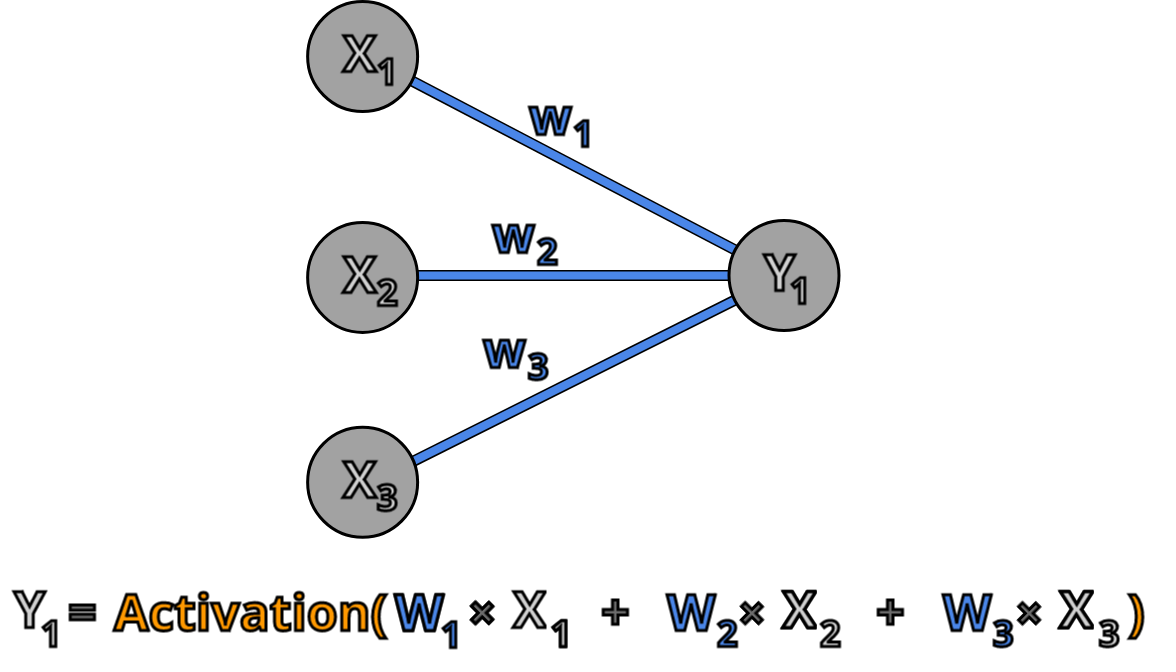
\includegraphics[width=10cm]{media/nn_formula.png}
		\cite{website:BH_AI}
	\end{figure}
	\newline
	
	Traditional Neural Networks also face an issue of handling sequential data, which is partly solved with Recurrent Neural Networks (RNN). RNN add a memory element to traditional Neural Networks, meaning that the output of the previous layers are remembered sequentially. The most common applications of RNN are within time series forecasting and natural language processing. The issue with RNN is that "they cannot learn long term dependencies due to vanishing gradients" \cite{website:AV_LSTM}, this occurs because the weights of the previous layers that are passed through each stage are multiplied which will always result in a smaller number, meaning the loss will decrease towards 0. Long Short Term Memory networks (LSTM) overcome this issue by introducing memory gates (Figure 2.2).
	\begin{figure}
		\caption{Long Short Term Memory network gates}
		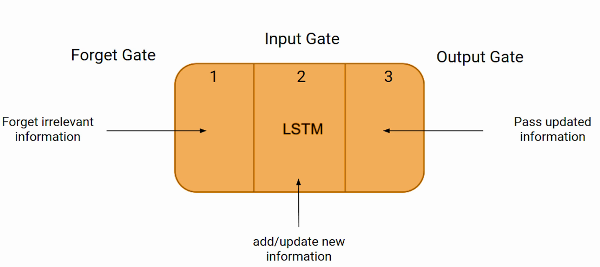
\includegraphics[width=15cm]{media/LSTM.png}
		\cite{website:AV_LSTM}
	\end{figure}
	The forget gate analyses the information from the previous time step, called the hidden state and decides whether it is important and should be kept of if it should be forgotten.
	The input gate is used to identify the importance of the current input values.
	The output gate determines the value of the hidden state which will be stored and analysed in the next time step.
	\newline
	
	After the model has been built and tuned to produce the best result, the Deployment and Monitoring phase can begin. 
	
	The first section of this paper will be the exploration of the data set with the aim of identifying trends and important features within the data. Important features are features that have a greater impact on the final result of a prediction model. Trends will be defined as features or feature patterns that occur in multiple seasons. Both known and unknown features and trends will be extracted and from the data set. Known features will be defined as factors that are currently used in analysis of sports games, which stem from less scientific analysis of data. These known features are generally used in predictions of games by both domain experts and casual observers and are widely accepted to be true, but there has been little research to provide evidence to the claims. The unknown features and trends will be discovered during the data exploration and will be represented by the important features, the factors which have the greatest effect on the outcome of the model, extracted during the feature engineering process.\newline
		
	In the analysis of AFL games there are many factors that are said to have an impact on results by domain experts and casual viewers alike, these factors will be analysed as known features in the data set. There are two main ideas behind exploring these features. Firstly, it is useful to take domain knowledge from experts, even if it second hand as in this case. Having access to expert domain knowledge can provide a solid foundation in data analysis workflows, it allows for the analysis to be applied in a specific area of the data set without the need for pre-analysis and feature extraction. The second reason is to statistically analyse whether there is any truth to these claims and if this analysis can be useful when used as a feature in a computer aided prediction model.
	\newline 
	
	The main points that will be explored from this expert analysis are the effects of weather conditions both during and in subsequent games, the length between games and the impacts of travel on future results. The impact of weather will be analysed in two features, the first being the impact of a previous games rainfall conditions as it is believed that it can negatively affect a team’s performance in future weeks, as the game becomes more contested thus requiring a greater physical output. The second will be the impact of rainfall on a current game, rainfall during games generally reduces disposal efficiency making results closer, and also different game plans are impacted more by rainfall thus it can be assumed that rainfall will have some correlation to specific teams (rainfall for the model will be taken as predicted rainfall, connected to teams). While with travel it is suggested that spending long times in planes both before and after games can affect a teams’ recovery and preparations. There has been research done on the impact of weather on team performance in the AFL\cite{website:AFL_Weather}, which focuses on the analysis of results as such the findings are not used to aid in any prediction models, which this paper aims to do.
	\newline
	
	While trends can be extremely useful for prediction they can also be difficult to interpret and extract from data. This is another reason why the expert analysis is being explored. It gives a starting point from which the data can be analysed. Basic visualisation of the data set will be used to asses the expert analysis. Further extraction of trends will be entirely theoretical and based solely on algorithmic interpretation of the data set. This will be very important for the project as it will hopefully enable hidden features to be found, rather than just proving or disproving already voiced opinions. These trends would be much more valuable in the industry as they would give professionals a completely new insight into their analytics.
	
	The final key section will be the implementation of a prediction model. Prediction models are used regularly in sports. However as there are so many unknown factors in these prediction models it is very difficult to explain their predictions and how they came to these decisions. The aim is to create a prediction model based on the extracted trends and important features, that is more explainable than other models. 
	Assuming that the prediction model does reliably work, one more key piece of information will be extracted, the final research question, what number of rounds/games does the model need before it can reliably predict the outcomes of games? This can be useful not only for this model but for other prediction models for the AFL, as it can give a greater understanding of when results and match data will stabilise and become reliable in defining the characteristics of a season. The general consensus is that after 4 - 6 weeks of matches is when a reliable data set begins to form.
	There are many algorithms and techniques that can be used in Data Mining and sports, this paper will mainly utilise the following:
	
	\begin{enumerate}
		\item[] Decision Trees: A tree like predictive models that shows where certain decisions were made via nodes.
		\item[] Random Forest: A collection of decision trees, that uses a random subset of the data in each iteration.
		\item[] Long Term Short Term Neural Networks (LSTM): A type Neural Network that introduces the concept of memory and feedback connections allowing it to process data sequences.
	\end{enumerate}
	

	
	\chapter{Method}\label{chap:method}
	\section{Description of the Scientific Method }
	
	\subsection{Technical Environment}
	0.5 pages
	The project will be completed using python as the main programming language. There will be numerous libraries used during the project, but they will be identified during implementation, at this stage it is impossible to know every library that will be used.
	
	\subsection{Phase 1: Data Acquisition}
	0.5 pages
	The dataset was taken from Kaggle (https://www.kaggle.com/datasets/stoney71/aflstats), it is a comprehensive dataset, containing statistics from every AFL game between 2012 and 2021. It is comprised of 3 tables, Games (containing game data) has 12 columns, Players (containing player information) has 7 columns, and Stats (containing individual player statistics for every game) has 31 columns. Overall there are over 90000 data points across the datasets.
	
	However there are some values that will be sourced from other websites to enhance the dataset, Fantasy Score and Supercoach Scores (player ratings after a game) will be taken from footywire.com. Travel time data will be manually updated. Days between games will be calculated via a python script in pre-processing.
	
	\subsection{Phase 2: Data Engineering}
	2 pages
	
	\subsection{Phase 3: Feature Engineering}
	3 pages
	The first phase of the paper is the Data Mining on the entire dataset using Regression and Random Forest models to extract important features and trends from the dataset. This is central to answering the first research question, can data mining be used to find, key features and patterns and explain results in professional sports?
	These models will be built on the entire featured dataset in multiple independent tests utilising different sections on the data. The main focus will be on the games table as it will be used in the second model, the experimentation on the other tables will be done to extract importance values for individual player data and team selection.
	Each player will have a performance score calculated for each game based on table 1.
	The importance values will be a standardised value between 1 and 10. It will be calculated using a players previous 5 games with most recent games having higher weights (1, 0.8, 0.6, 0.4, 0.2) and diving it by 3 (the sum of the weights) and added to the games table as “Home Team Player Importance” and “Away Team Player Importance”
	\begin{table}[h!]
		\centering	
		\begin{tabular}{| c | c |}
			\hline
			Stat & Value +/- \\
			\hline
			Kick & 4 \\
			\hline
			Handball & 2 \\
			\hline
			Mark & 3 \\
			\hline
			Goal & 6 \\
			\hline
			Behind & 1 \\
			\hline
			Hitout & 2 \\
			\hline
			Tackles & 3 \\
			\hline
			Rebounds & 1 \\
			\hline
			Inside 50s & 2\\
			\hline
			Clearances & 3 \\
			\hline
			Clangers & -3 \\
			\hline
			Free Against & -3 \\
			\hline
			Contested Marks & 3 \\
			\hline
			One Percenters & 3 \\
			\hline
			Goal Assist & 2 \\
			\hline
		\end{tabular}
		\caption{\label {tab:PlayerImportance}Players count for each stat is multiplied by the value.}
		
	\end{table}
	
	Once the values have been defined the model can be built and trained. 
	For testing a new table will be created building on the games table. It will contain a combination of the features: Disposals, Kicks, Handballs, Tackles, Free Kicks, Hit Outs, Contested Possessions, Player Importance, Marks, Contested Marks, Inside 50s, Rebounds, Clangers, Team Name, Travel Distance and Break Between Games for both teams as well as Rainfall. This will try to predict which team won. 20 percent of the data will be held out for testing purposes.
	
	Evaluation in this phase is the feature importance metrics. Random Forests will be used for finding feature importance as they are naturally capable of discerning important features. 
	Ideally 5 features would be identified that consistently are found to have the greatest impact on predicting the result of a model and the 5 features that consistently have the least impact on the result. To realise this outcome a random forest model containing 100 trees and the 5 metrics that were found most and least important on average will be taken as the fitting metrics.
	
	
	\subsection{Phase 4: Predictive Model}
	3 pages
	The second phase has to do with the building of a prediction model, using the knowledge of important features gained from the previous phase.
	The prediction model will be created using a LTSM Neural Network. The data acquisition and pre-processing will be much shorter as the majority had been done previously in the first phase of the project. Again a table will be built that is similar to the table used in the random forest model. However, the 5 least important features will be removed (and the corresponding feature for the opposite team). The scores of the home and away team will be included in the dataset as well as the round number and year.
	The dataset will then be separated by year and ordered by the round.
	Because the model will be predicting future events the training and test data split will not be static. The initial tuning phase will hold out only the final round, making the model theoretically as powerful as possible. But in different iterations more or less rounds will be held out, this is crucial to see if there is a certain point where the models begin to see an increase in their predictive powers.
	Evaluation on the models 
	The main metric I will use to evaluate my model is the Mean Average Percentage Error (MAPE), which is “the proportion of the average absolute difference between projected and true values divided by the true value” \cite{website:AIM}, and the Weighted Mean Average Percentage Error (WMAPE) will be used if the dataset is too small to calculate the MAPE properly. Previous prediction models utilising machine learning have been able to reach a best accuracy of 68.1 percent and average accuracy of 65.1 percent \cite{AFL_1}. Knowing that models are capable of reaching these accuracies, the target accuracy of the prediction model will be greater than those values, ideally above 70 percent.
	
	\chapter{Results and Discussion}\label{chap:Results}
	
	\subsection{EDA Results}
	
	\subsection{Feature Engineering Results}
	
	\subsection{Final Model Results}
	
	\chapter{Related Works}\label{chap:related_works}
	\subsection{Data Mining}
	Although data mining is not a big subject in sports it is a major influence in many other industries. Data Mining has a very broad use case in both Supervised and Unsupervised learning. Supervised learning is a subcategory of machine learning that deals with data where the input and output is known, as is the case with the data in this paper, it aims to map input data to resulting output data. Supervised learning can be further divided into two categories Classification, where the output is a class or category and Regression where the output is continuous. 
	
	There are many state of the art data mining techniques in both Classification and Regression. There have been some Classification Methods already mentioned in the paper, Decision Trees and Neural. Other widely used algorithms include K Nearest Neighbour (KNN), Support Vector Machines (SVM) and Bayesian Methods \cite{SOTA}. The K Nearest Neighbours attempts to classify a data point based on the class of its Nearest Neighbour points, a SVM is a method that aims to define boundaries to separate a space into classes. Bayesian Methods are more complex it is based upon a method that “combines prior information about a population parameter with new evidence from information contained in a sample to guide the statistical inference process” \cite{website:Britannica}, the basis of the inference is gained through an application of Bayes Theorem \cite{website:Britannica}. The main application of these algorithms is to forecast how a certain input will act based on their characteristics, in the finance industry this can be deciding how likely a customer is to default on their payments based on their previous behaviours, in the medical industry these can be used to predict how likely a patient is to have a certain medical condition.
	
	\subsection{Long Short Term Memory Networks}	
	The state of the art of Long Short Term Memory networks is very centralised around stock market predictions and natural language processing, with some forays into image and video analysis. 
	Time series forecasting, techniques, similar different
	Time Series \cite{10.1145/3453800.3453812}
	
	Stock market predictions, techniques, similarities 
	Indonesia\cite{10.1145/3568231.3568249}
	Bitcoin \cite{10.1145/3546157.3546162}
	Dividend \cite{10.1145/3474880.3474898}
	
	Natural language processing, techniques, similarities, 
	Sentence Embedding \cite{10.1109/TASLP.2016.2520371}
	Spam \cite{10.1145/3234781.3234794}
	
	\subsection{Data Mining in Sports}
	Although there are many state of the art use cases of data mining, they have limited use in the field of sports. As discussed in “Sports Data Mining” by Robert P. Schumaker et al. \cite{SportDM}. This text looks at which data should be collected to properly performing data mining in sports and “how to best make use of it”. It also discusses the issues faced by those entering data mining in sports not only in the initial phases but also the final phases of data mining. One of these difficulties is the relationships between sports organisations and their data, many were unwilling to embrace data mining techniques at the time of the publication of the book. They defined 5 levels of relationships between organisations and the data they produced. Shown below in table 2, taken from Chapter 1, page 2 from the book.
	
	\begin{table}[h!]
		\centering	
		\begin{tabular}{| c | c |}
			\hline
			Level & Relationship\\
			\hline
			One & No relationship \\
			\hline
			Two & Human domain experts make predictions using instinct and gut feeling \\
			\hline
			Three & Human domain experts make predictions using historical data \\
			\hline
			Four & Use of statistics in the decision-making process \\
			\hline
			Five & Use of data mining in the decision-making process  \\
			\hline			
		\end{tabular}
		\caption{\label {tab:Sport Data Relation}Hierarchy of Sport and Sport Data Relationships.}		
	\end{table}
	
	Schumaker claims in the text that at the time of publishing many organisations resided in level 3 or 4 of the hierarchy.  The issue is that there is currently no straightforward way to identify if organisations are using data mining and how they are using it. 
	Another issue highlighted in the text is the inconsistencies and misinterpretations of statistical sports data. As is pointed out in the text many long standing statistics are misleading in modern contexts where we now have a better grasp on these methods and much greater available computing abilities. However, these methods still remain prominent and in use today, as such the book seeks to define new methods to ensure proper algorithms and applications of data analysis and data mining are used. 
	In the book the Data-Information-Knowledge-Wisdom Hierarchy (DIKW) is used to separate techniques and use cases into each of the categories, to identify the best methods and algorithms to be used on each use case. 
		
	Moving into the field of academic papers there are only a handful of resources that explore similar issues to this paper. The most common areas of focus are American Football, Basketball and Baseball. 
	
	Carson Leung and Kyle Joseph, explore a prediction model for American Football in their paper, “Sports Data Mining: Predicting results for the college football” \cite{CollegeFootball}. They employ an interesting dropout technique for their prediction model, in which they do not explore the results of the two teams that will be predicted, instead focusing on “a set of teams that are the most similar to each of the competing teams” \cite{CollegeFootball}, [page 716]. Similarly, they identify statistics on which the final model will be based, but only 4 instead of the larger set as in the model in this paper.
	
	On the more analytical side is the paper “Sports analytics— Evaluation of basketball players and team” by Vangelis Sarlis and corresponding author Christos Tjortjis. This paper looks at and “evaluates the existing performance analytics used in Europe and NBA (in USA) basketball” \cite{Basketball}. They identify two metric types, Player and Team, and four criteria groups; Key Performance Indicators (KPIs), Defensive criteria, Offensive Criteria and Overall Performance Criteria, as well as outlining a Comparison Matrix and Data Mining Techniques used in sports analysis. They also explore if they can optimise existing performance analysis metrics that are used in basketball. 
	
	An overall review of the current techniques used in sports prediction (as of 2013) is given in the paper “A review of Data Mining Techniques for Result Prediction in Sports”, M. Haghighat et al., \cite{ResearchGate}. 6 Methods are analysed in the resource of which two, Artificial Neural Networks and Decision Trees are used in this paper. Bayesian Method, Logistic Regression, Support Vector Machines and Fuzzy Methods are the other methods that are analysed. Since nearly 10 years have passed since this resource was published, there has been many improvements to the models that are used in this paper, specifically in the field of Neural Networks. 
	
	Very little comprehensive work has been completed regarding Data Science and Australian Football. In 2008 McCabe and Travathan briefly explored the usability of neural networks in predicting the outcomes of sports in their conference paper “Artificial Intelligence in Sports Prediction” \cite{AFL_1}. Here they reached an average accuracy of 65 percent using 11 performance metrics. Other studies conducted on AFL data include “Using meta-regression data mining to improve predictions of performance based on heart rate dynamics for Australian football” \cite{AFL_2}, which focuses on individual player performance as opposed to team performance prediction, but does follow a similar scientific method, utilising Random Forest algorithms to extract key features from the dataset, which is more complex featuring GPS data on top of more traditional performance measures. Also utilising GPS data is “The effect of team formation on defensive performance in Australian \cite{AFL_3}, which analysed a team’s defensive positioning and the effect it had on defensive performance. These both used similar techniques but the dataset differed from what will be used in this paper.
	
	Sports ML \cite{BUNKER201927}
	
	Human Activity Modelling \cite{10.1145/3316782.3322781}
	
	\newpage
	\chapter{Summary}\label{chap:summary}
	\section{Summary}
	Overall this paper intends to expand the understanding and use of Data Mining in Professional Sports, specifically the Australian Football League. It aims to combine and build upon methods already being used in sports data mining to explore the following research questions:
	\begin{enumerate}
		\item[] Can data mining be used to find key features and patterns and explain results in professional sports?
		\item[] Can these extracted trends and features be used to create an explainable prediction model?
		\item[] How can the results be utilised in the sporting industry?
		\item[] If the model can reliably predict outcomes, how many rounds will the model need before it becomes reliable?
	\end{enumerate}
	In the paper Decision Trees, Random Forests, Linear Regression Models and LSTM Neural Networks will be utilised to extract important features and trends in the Australian Football League and use them to implement an explainable prediction model.
	
	A two phase approach will be taken to create the final model. The first being feature engineering and trend analysis, using the Decision Tree and Random Forest techniques and Linear Regression. This will be done iteratively until the 5 most important and least important features are identified. The second phase will be the building of the prediction model, utilising the results from the first phase, with the aim of achieving an average accuracy greater than 65.1 percent.
	
	
	\newpage
	\bibliography{refs_thesis} %name of the .bib file
	\bibliographystyle{ieeetr}
	
\end{document}


\section{Adding images}
Adding a simple image is easy. Adding complex images is also easy. What is a complex image anyway? 
\begin{figure}[h]
	\centering
	
\includegraphics[width=1.0\textwidth]{imclogo.png}
	\caption{IMC Logo}
	\label{fig:logo}
\end{figure}





\begin{figure}[ht]
	\begin{subfigure}{.5\textwidth}
		\centering
		% include first image
		
\includegraphics[width=.8\linewidth]{imclogo.png}  
		\caption{Put your sub-caption here}
		\label{fig:sub-first}
	\end{subfigure}
	\begin{subfigure}{.5\textwidth}
		\centering
		% include second image
		
\includegraphics[width=.8\linewidth]{imclogo.png}  
		\caption{Put your sub-caption here}
		\label{fig:sub-second}
	\end{subfigure}
	\caption{Including sub images! }
	\label{fig:fig}
\end{figure}

\section{Tables}

\begin{table}[ht]
	\begin{tabular}{ |p{3cm}||p{3cm}|p{3cm}|p{3cm}|  }
		\hline
		\multicolumn{4}{|c|}{Country List} \\
		\hline
		Country Name     or Area Name& ISO ALPHA 2 Code &ISO ALPHA 3 Code&ISO numeric Code\\
		\hline
		Afghanistan   & AF    &AFG&   004\\
		Aland Islands&   AX  & ALA   &248\\
		Albania &AL & ALB&  008\\
		Algeria    &DZ & DZA&  012\\
		American Samoa&   AS  & ASM&016\\
		Andorra& AD  & AND   &020\\
		Angola& AO  & AGO&024\\
		\hline
	\end{tabular}
	\caption{\label{tab:table-name}Example table}
\end{table}


\backmatter%
\addtoToC{Bibliography}
\bibliographystyle{IEEEtran}
\bibliography{refs_thesis}


\begin{appendices} % optional
	\chapter{Example Appendix 1}
	
	Appendices should be used for supplemental information that does not form part of the main research. Remember that figures and tables in appendices should not be listed in the List of Figures or List of Tables. 
	
	\chapter{Example Appendix 2}
	
	Appendices should be used for supplemental information that does not form part of the main research. Remember that figures and tables in appendices should not be listed in the List of Figures or List of Tables. 
	
\end{appendices}
\end{document}